% =====================================================================
% Extensão: 2 novos datasets (COVID19.BR e FACTCK.BR).
% Arquivo novo timestamped (20261026T064945Z); NÃO sobrescreve os .tex/.pdf existentes.
% Metodologia idêntica à revisão 21/out v2 (estudo controlado de curadoria).
% =====================================================================
\documentclass[conference]{IEEEtran}
\usepackage[utf8]{inputenc}
\usepackage[T1]{fontenc}
\usepackage{cite}
\usepackage{amsmath,amssymb,amsfonts}
\usepackage{graphicx}
\usepackage{textcomp}
\usepackage{xcolor}
\usepackage{booktabs}
\usepackage[hidelinks]{hyperref}
\usepackage{url}
\usepackage{balance}
\graphicspath{{./images/}{../figures/revision/}{./}}
\setlength{\textfloatsep}{6pt plus 1pt minus 1pt}
\setlength{\intextsep}{5pt plus 1pt minus 1pt}
\setlength{\floatsep}{5pt plus 1pt minus 1pt}
\widowpenalty=10000
\clubpenalty=10000

\begin{document}

\title{Gera\c{c}\~ao Sint\'etica Guiada por Heran\c{c}a Ativa: Extens\~ao Multi-dom\'inio (COVID19.BR e FACTCK.BR)}

\author{\IEEEauthorblockN{Eduardo Alexandre de Amorim\textsuperscript{1}, Cleber Zanchettin\textsuperscript{1}}
\IEEEauthorblockA{\textsuperscript{1}Centro de Inform\'atica, Universidade Federal de Pernambuco, Recife, PE, Brasil\\
\{eaa5, cz\}@cin.ufpe.br}}

\maketitle

\begin{abstract}
Esta extens\~ao replica o estudo controlado de curadoria da revis\~ao 21/out em dois novos dom\'inios do portugu\^es: COVID19.BR (mensagens de WhatsApp sobre a pandemia, split temporal) e FACTCK.BR (claims verificados por ag\^encias de checagem, split aleat\'orio estratificado). Dados os mesmos candidatos zero-shot, quatro regras de heran\c{c}a s\~ao comparadas---herdar tudo (\emph{All}), uma amostra aleat\'oria (\emph{Random-}k), o score de erro/incerteza/diversidade (\emph{Score-}k) e o gate invertido (\emph{Easy-}k)---em tr\^es cen\'arios de escassez por dom\'inio (full, 10\%, 5\%). Todos os bra\c{c}os usam pondera\c{c}\~ao de classes, limiar ajustado na valida\c{c}\~ao e treino final do zero. Os resultados (tr\^es seeds, explorat\'orio) s\~ao reportados com F1, recall, PR-AUC e custo; nenhum resultado hist\'orico foi sobrescrito.
\end{abstract}

\begin{IEEEkeywords}
data-centric AI, synthetic data, misinformation, controlled study, Portuguese NLP, COVID19.BR, FACTCK.BR
\end{IEEEkeywords}

\section{Introdu\c{c}\~ao}

A revis\~ao 21/out isolou tr\^es efeitos confundidos na vers\~ao anterior do \emph{ActiveInheritance}: o score de sele\c{c}\~ao, o volume gerado e a pol\'itica de treino (limiar fixo $0{,}5$ sem pondera\c{c}\~ao). O achado central foi que, dados os mesmos candidatos, o score \textbf{n\~ao} domina a sele\c{c}\~ao aleat\'oria, e que boa parte do colapso de recall sob escassez era efeito do limiar e do desbalanceamento. Aquela an\'alise, por\'em, usou um \'unico dom\'inio novo (FakeWhatsApp.Br). Aqui estendemos o mesmo protocolo a dois dom\'inios adicionais para verificar se a conclus\~ao se mant\'em fora de WhatsApp eleitoral.

\section{Datasets}

Os quatro dom\'inios do estudo diferem em g\^enero, pr\'e-processamento, prior de classe e tipo de split (Tabela~\ref{tab:datasets}). Os dois primeiros v\^em da revis\~ao 21/out; os dois \'ultimos s\~ao as contribui\c{c}\~oes desta extens\~ao.

\begin{table}[t]
\caption{Caracter\'isticas dos quatro dom\'inios do estudo.}\label{tab:datasets}
\centering
\begin{tabular}{lllll}
\toprule
Dom\'inio & G\^enero & Texto & Prior (fake:true) & Split \\
\midrule
Fake.br & not\'icia & pr\'e-processado & balanceado & aleat\'orio \\
FakeWhatsApp.Br & WhatsApp & raw & minorit\'ario & temporal \\
COVID19.BR & WhatsApp & raw & minorit\'ario ($\approx$1:2{,}5) & temporal \\
FACTCK.BR & claims & raw & majorit\'ario & aleat\'orio estrat. \\
\bottomrule
\end{tabular}
\end{table}

\subsection{COVID19.BR}

Mensagens reais de grupos p\'ublicos brasileiros de WhatsApp durante a pandemia de COVID-19 (mar\c{c}o--junho/2020), rotuladas manualmente como misinformation. Vem da mesma fam\'ilia do FakeWhatsApp.Br (mesmo grupo de pesquisa e mesmo esquema \texttt{text}/\texttt{misinformation}), o que garante texto \emph{raw} nos dois lados---sem o descompasso real-pr\'e-processado\,vs.\,sint\'etico que limitava o Fake.br. O split \'e temporal (treino=mar\c{c}o--abril; valida\c{c}\~ao=08--09/junho; teste=10--12/junho): o teste mede generaliza\c{c}\~ao para um per\'iodo posterior da pandemia, e n\~ao apenas para uma subamostra aleat\'oria. A classe \texttt{fake} \'e naturalmente minorit\'aria ($\approx$1:2{,}5), exatamente o regime de escassez para o qual o m\'etodo foi desenhado.

\subsection{FACTCK.BR}

Claims verificados por ag\^encias brasileiras de checagem (Aos Fatos, Lupa, Truco), coletados via schema ClaimReview entre 2016 e 2019. \'E um g\^enero distinto: alega\c{c}\~oes curtas, n\~ao mensagens nem artigos completos. O texto usado \'e o \texttt{claimReviewed} (a pr\'opria alega\c{c}\~ao); o \texttt{reviewBody} foi exclu\'ido porque declara o veredito e vazaria o r\'otulo. A binariza\c{c}\~ao \'e estrita (falso/falsa\,$\to$\,fake; verdadeiro/verdadeira\,$\to$\,true; demais r\'otulos descartados). O split \'e aleat\'orio estratificado 70/15/15 (seed 42): o temporal foi evitado porque os claims \texttt{true} se concentram em 2016--2018, deixando 2019 sem classe negativa. Diferentemente dos demais, \'e \emph{fake-majorit\'ario} (ag\^encias checam majoritariamente claims falsos), servindo como teste de robustez a um prior oposto.

\section{Protocolo}

Id\^entico ao da revis\~ao 21/out: uma gera\c{c}\~ao zero-shot por cen\'ario/seed (\texttt{candidates.json}) e quatro replays offline sobre os \emph{mesmos} lotes. \texttt{deepseek-chat}, prompt v4 (WhatsApp anti-template) para COVID19.BR e prompt v2 (not\'icia) para FACTCK.BR, teto de 100 mil tokens por gera\c{c}\~ao, $T{=}5$, batch 64, top-$k{=}16$. Learner BERTimbau, 3 \'epocas por fit, pondera\c{c}\~ao de classes e limiar na valida\c{c}\~ao; treino final do zero em $D_0\cup H$. Seeds 42--44 ($n{=}3$, explorat\'orio).

\section{Resultados}

Tabela~\ref{tab:f1} reporta F1 (m\'edia\,$\pm$\,desvio) por dom\'inio, cen\'ario e bra\c{c}o. Tabela~\ref{tab:aux} traz recall, PR-AUC, limiar e n\'umero de sint\'eticos herdados.

\begin{table}[t]
\caption{F1 (teste) por dom\'inio, cen\'ario e bra\c{c}o. $n{=}3$ seeds.}\label{tab:f1}
\centering
\begin{tabular}{llcccc}
\toprule
Dom\'inio & Cen. & All & Random-k & Score-k & Easy-k \\
\midrule
COVID19.BR & full & 0.824 $\pm$ 0.024 & 0.836 $\pm$ 0.013 & 0.857 $\pm$ 0.003 & 0.848 $\pm$ 0.013 \\
COVID19.BR & 10\% & 0.789 $\pm$ 0.017 & 0.732 $\pm$ 0.049 & 0.805 $\pm$ 0.018 & 0.773 $\pm$ 0.041 \\
COVID19.BR & 5\% & 0.468 $\pm$ 0.029 & 0.704 $\pm$ 0.039 & 0.668 $\pm$ 0.062 & 0.601 $\pm$ 0.133 \\
FACTCK.BR & full & 0.929 $\pm$ 0.004 & 0.931 $\pm$ 0.006 & 0.932 $\pm$ 0.010 & 0.926 $\pm$ 0.003 \\
FACTCK.BR & 10\% & 0.816 $\pm$ 0.044 & 0.931 $\pm$ 0.011 & 0.934 $\pm$ 0.007 & 0.937 $\pm$ 0.008 \\
FACTCK.BR & 5\% & 0.765 $\pm$ 0.076 & 0.928 $\pm$ 0.010 & 0.935 $\pm$ 0.006 & 0.931 $\pm$ 0.006 \\
\bottomrule
\end{tabular}
\end{table}

\begin{table}[t]
\caption{Recall, PR-AUC, limiar e sint\'eticos herdados (m\'edia).}\label{tab:aux}
\centering
\begin{tabular}{llcccc}
\toprule
Dom\'inio & Cen. & Bra\c{c}o & Recall & PR-AUC & n\_synth \\
\midrule
COVID19.BR & full & all & 0.802 & 0.886 & 277 \\
COVID19.BR & full & random-k & 0.822 & 0.897 & 80 \\
COVID19.BR & full & score-k & 0.871 & 0.901 & 80 \\
COVID19.BR & full & easy-k & 0.853 & 0.907 & 80 \\
COVID19.BR & 10\% & all & 0.791 & 0.853 & 278 \\
COVID19.BR & 10\% & random-k & 0.653 & 0.848 & 80 \\
COVID19.BR & 10\% & score-k & 0.789 & 0.853 & 80 \\
COVID19.BR & 10\% & easy-k & 0.731 & 0.861 & 80 \\
COVID19.BR & 5\% & all & 0.322 & 0.792 & 278 \\
COVID19.BR & 5\% & random-k & 0.660 & 0.818 & 80 \\
COVID19.BR & 5\% & score-k & 0.591 & 0.801 & 80 \\
COVID19.BR & 5\% & easy-k & 0.498 & 0.806 & 80 \\
FACTCK.BR & full & all & 0.959 & 0.971 & 313 \\
FACTCK.BR & full & random-k & 0.969 & 0.968 & 80 \\
FACTCK.BR & full & score-k & 0.966 & 0.965 & 80 \\
FACTCK.BR & full & easy-k & 0.952 & 0.967 & 80 \\
FACTCK.BR & 10\% & all & 0.734 & 0.961 & 312 \\
FACTCK.BR & 10\% & random-k & 0.978 & 0.961 & 80 \\
FACTCK.BR & 10\% & score-k & 0.986 & 0.961 & 80 \\
FACTCK.BR & 10\% & easy-k & 0.986 & 0.963 & 80 \\
FACTCK.BR & 5\% & all & 0.657 & 0.952 & 312 \\
FACTCK.BR & 5\% & random-k & 0.969 & 0.955 & 80 \\
FACTCK.BR & 5\% & score-k & 0.988 & 0.957 & 80 \\
FACTCK.BR & 5\% & easy-k & 0.978 & 0.960 & 80 \\
\bottomrule
\end{tabular}
\end{table}

\section{Discuss\~ao}

Os resultados confirmam e refinam a conclus\~ao da revis\~ao 21/out em dois dom\'inios novos, com quatro insights principais.

\textbf{(i) O score n\~ao domina --- e o controle aleat\'orio continua sendo a barreira.} No COVID19.BR, \emph{Score-}k s\'o vence \emph{Random-}k no cen\'ario full (0{,}857 vs.\ 0{,}836) e por margem pequena; sob escassez, \emph{Random-}k empata ou vence (5\%: 0{,}704 vs.\ 0{,}668). No FACTCK.BR os quatro bra\c{c}os ficam praticamente empatados em todos os cen\'arios. Dados os mesmos candidatos, o score de erro/incerteza/diversidade n\~ao agrega sobre uma sele\c{c}\~ao aleat\'oria.

\textbf{(ii) O efeito real \'e curadoria de volume, n\~ao o score.} \emph{All} herda 277--313 sint\'eticos; os demais herdam $\approx$80. Em escassez extrema (COVID19.BR 5\%), \emph{All} colapsa para F1 0{,}468 enquanto os bra\c{c}os curados ficam em 0{,}60--0{,}70. Herdar \emph{menos} e manter o treino rebalanceado importa mais do que \emph{o qu\^e} se herda.

\textbf{(iii) A sele\c{c}\~ao s\'o agrega num regime intermedi\'ario de dificuldade --- quando o learner inicial j\'a \'e bom.} No FACTCK.BR a tarefa \'e f\'acil (\emph{All} j\'a alcan\c{c}a 0{,}929 no full) e a regra de sele\c{c}\~ao se torna irrelevante: os quatro bra\c{c}os empatam. No COVID19.BR 5\% a tarefa \'e dif\'icil (\emph{All} colapsa para 0{,}468) e o score tamb\'em n\~ao ajuda---\emph{Random-}k vence. S\'o no COVID19.BR full, dificuldade intermedi\'aria (\emph{All}=0{,}824), o score agrega um pouco (0{,}857). Isso ecoa o achado do Fake.br e do FakeWhatsApp.Br: a heran\c{c}a guiada pressup\~oe um learner suficientemente competente; quando ele \'e fraco, seu pr\'oprio sinal de erro/incerteza \'e ru\'ido e n\~ao supera o sorteio.

\textbf{(iv) Calibra\c{c}\~ao (pesos + limiar) continua fazendo o trabalho pesado.} Os limiares escolhidos na valida\c{c}\~ao caem para 0{,}05--0{,}11 nos cen\'arios de escassez: sem pondera\c{c}\~ao de classes e limiar ajustado, o modelo subestima a classe minorit\'aria e o recall colapsa (efeito j\'a documentado na revis\~ao). Boa parte do F1 observado \'e pol\'itica de treino, n\~ao qualidade intr\'inseca do sint\'etico.

\section{Figuras}

Fronteiras Pareto de F1\,$\times$\,tokens e F1\,$\times$\,n\_sint\'eticos para os cen\'arios completos:
\begin{figure}[t]
\centering
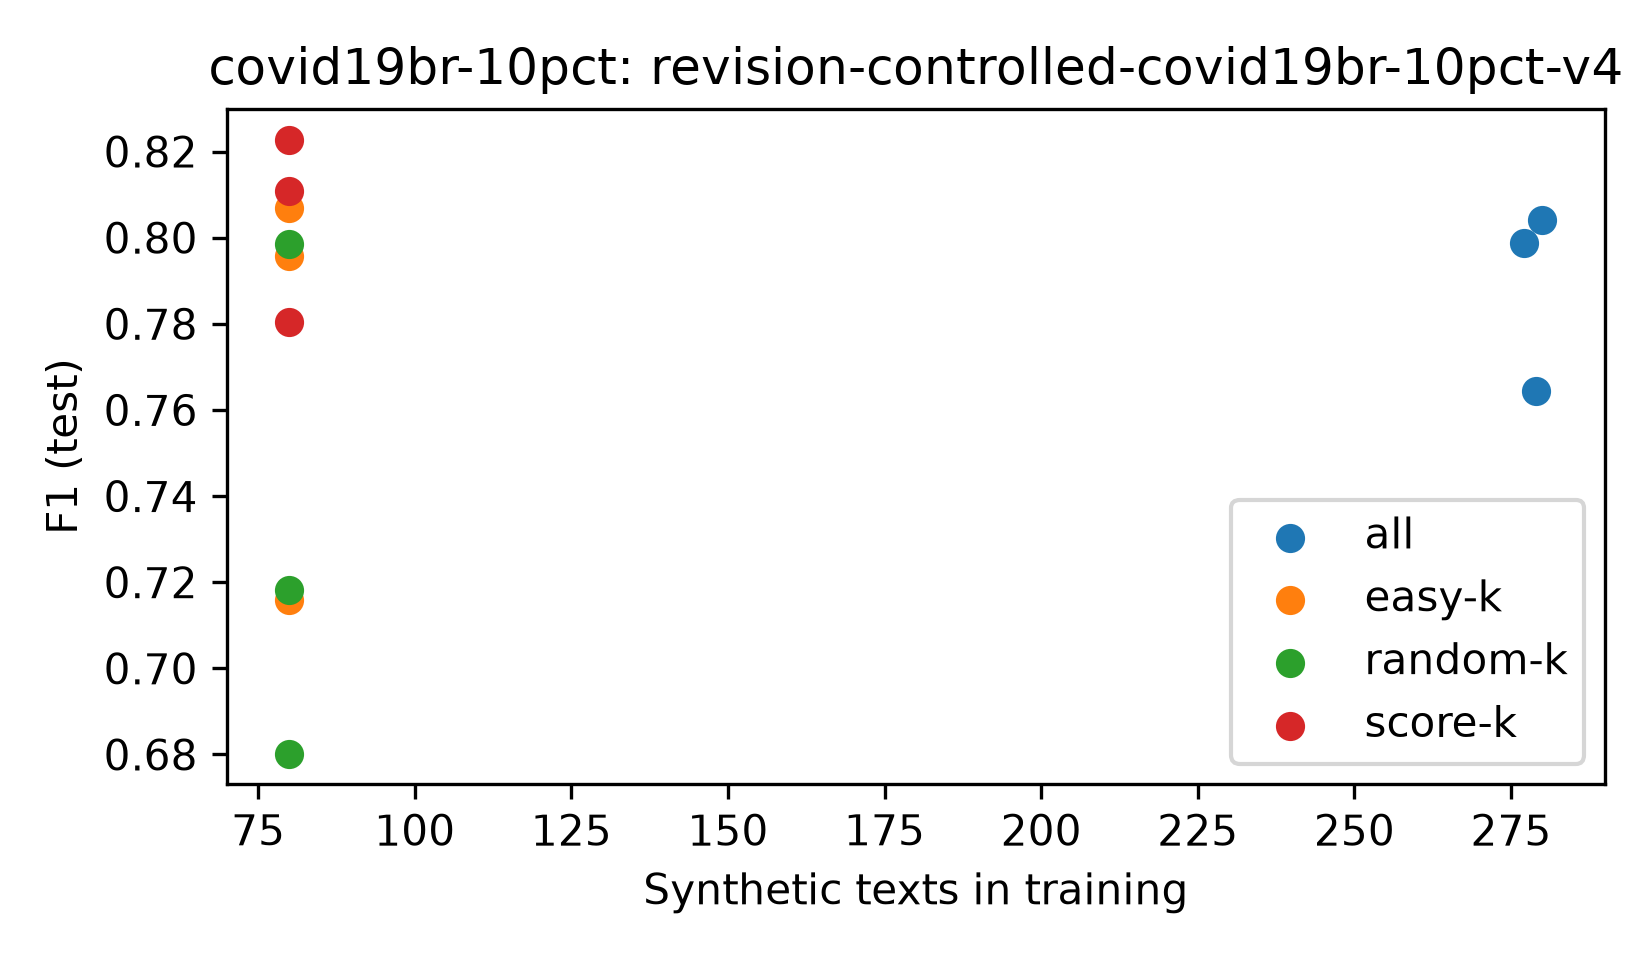
\includegraphics[width=\columnwidth]{revision-controlled-covid19br-10pct-v4-covid19br-10pct-f1-vs-n_synthetic-20261026T064951Z.png}
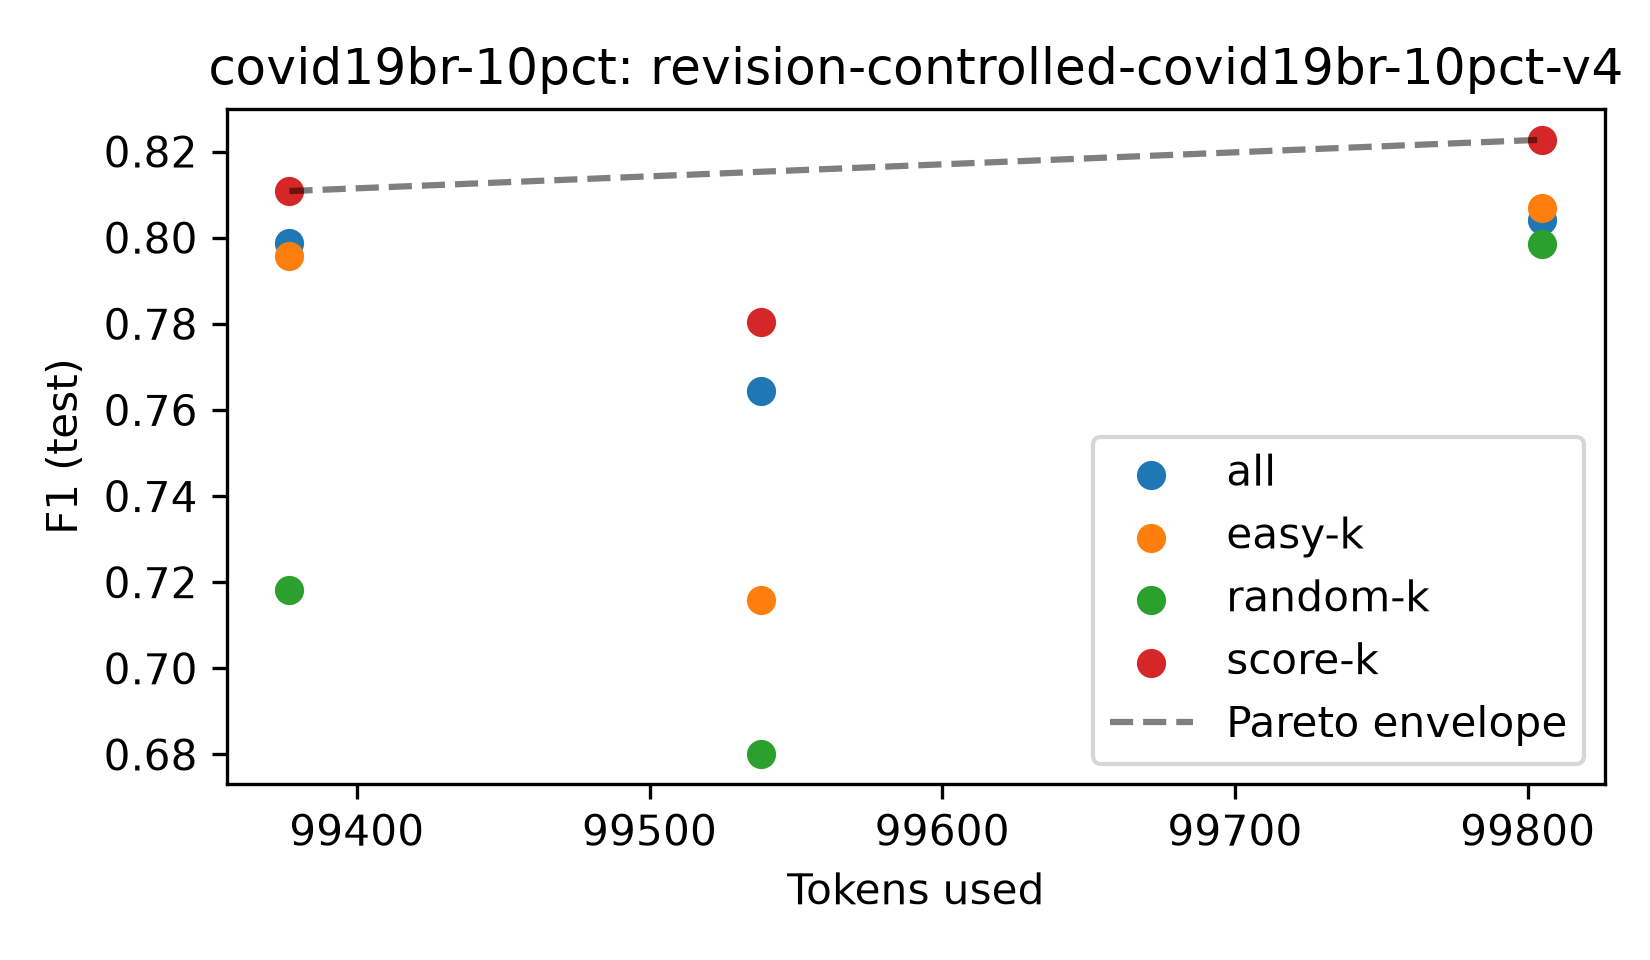
\includegraphics[width=\columnwidth]{revision-controlled-covid19br-10pct-v4-covid19br-10pct-f1-vs-tokens_used-20261026T064951Z.png}
\caption{Pareto F1\,$\times$\,recursos (cen\'ario full).}\label{fig:pareto}
\end{figure}

Figuras adicionais (todos os cen\'arios):
\begin{itemize}
\item \texttt{revision-controlled-covid19br-10pct-v4-covid19br-10pct-f1-vs-n\_synthetic-20261026T064951Z.png}
\item \texttt{revision-controlled-covid19br-10pct-v4-covid19br-10pct-f1-vs-tokens\_used-20261026T064951Z.png}
\item \texttt{revision-controlled-covid19br-5pct-v4-covid19br-5pct-f1-vs-n\_synthetic-20261026T064952Z.png}
\item \texttt{revision-controlled-covid19br-5pct-v4-covid19br-5pct-f1-vs-tokens\_used-20261026T064952Z.png}
\item \texttt{revision-controlled-covid19br-full-v4-covid19br-full-f1-vs-n\_synthetic-20261026T064946Z.png}
\item \texttt{revision-controlled-covid19br-full-v4-covid19br-full-f1-vs-tokens\_used-20261026T064946Z.png}
\item \texttt{revision-controlled-factckbr-10pct-v2-factckbr-10pct-f1-vs-n\_synthetic-20261026T064955Z.png}
\item \texttt{revision-controlled-factckbr-10pct-v2-factckbr-10pct-f1-vs-tokens\_used-20261026T064955Z.png}
\item \texttt{revision-controlled-factckbr-5pct-v2-factckbr-5pct-f1-vs-n\_synthetic-20261026T064956Z.png}
\item \texttt{revision-controlled-factckbr-5pct-v2-factckbr-5pct-f1-vs-tokens\_used-20261026T064956Z.png}
\item \texttt{revision-controlled-factckbr-full-v2-factckbr-full-f1-vs-n\_synthetic-20261026T064953Z.png}
\item \texttt{revision-controlled-factckbr-full-v2-factckbr-full-f1-vs-tokens\_used-20261026T064953Z.png}
\item \texttt{revision-controlled-fakewhatsapp-10pct-v4-fakewhatsapp-10pct-f1-vs-n\_synthetic-20261023T003530Z.png}
\item \texttt{revision-controlled-fakewhatsapp-10pct-v4-fakewhatsapp-10pct-f1-vs-tokens\_used-20261023T003530Z.png}
\item \texttt{revision-controlled-fakewhatsapp-5pct-v4-fakewhatsapp-5pct-f1-vs-n\_synthetic-20261023T003531Z.png}
\item \texttt{revision-controlled-fakewhatsapp-5pct-v4-fakewhatsapp-5pct-f1-vs-tokens\_used-20261023T003531Z.png}
\item \texttt{revision-controlled-fakewhatsapp-full-v4-fakewhatsapp-full-f1-vs-n\_synthetic-20261023T003526Z.png}
\item \texttt{revision-controlled-fakewhatsapp-full-v4-fakewhatsapp-full-f1-vs-tokens\_used-20261023T003526Z.png}
\end{itemize}

\section{Limita\c{c}\~oes}

\begin{itemize}
\item FACTCK.BR usa split aleat\'orio (n\~ao temporal) e prior invertido (fake majorit\'aria); n\~ao comparar diretamente com FakeWhatsApp.Br/COVID19.BR sem ressalvar.
\item FACTCK.BR \'e pequeno (\ensuremath{\approx}1.0k claims ap\'os binariza\c{c}\~ao); a classe \texttt{true} no teste \'e escassa (\ensuremath{\approx}18 exemplos).
\item COVID19.BR n\~ao tem dados em maio/2020; o teste \'e um futuro curto (junho).
\item $n{=}3$ seeds; n\~ao declarar signific\^ancia estat\'istica.
\item R\'otulos sint\'eticos s\~ao assumidos \texttt{fake} sem checagem humana; veracidade exige evid\^encia externa.
\end{itemize}

\balance
\end{document}